\section{SPH Equation}

\subsection{Euler Discription and Lagrangian Discription in Continuum Mechanics}

Contrary to traditional CFD method, 
SPH is proposed based on Lagrangian discription in continuum mechanics.
In Lagrangian discription, 
the motion of a fluid particle is described by its position $\vec{x}$ and velocity $\vec{u}$.

Let's consider a physical quantity $\phi$ in a fluid particle. 
In Euler discription, 
the variation of $\phi$ is described by:
\begin{equation}
    \begin{aligned}
        \mathrm{d} \phi &= \frac{\partial \phi}{\partial t} \mathrm{d} t + \frac{\partial \phi}{\partial x} \mathrm{d} x + \frac{\partial \phi}{\partial y} \mathrm{d} y + \frac{\partial \phi}{\partial z} \mathrm{d} z\\
        &=
        \frac{\partial \phi}{\partial t} \mathrm{d} t +
        \left(
        \frac{\partial \phi}{\partial x} \frac{\mathrm{d} x}{\mathrm{d} t} +
        \frac{\partial \phi}{\partial y} \frac{\mathrm{d} y}{\mathrm{d} t} +
        \frac{\partial \phi}{\partial z} \frac{\mathrm{d} z}{\mathrm{d} t}
        \right) \mathrm{d} t\\
        &\rightarrow\\
        \frac{\mathrm{d} \phi}{\mathrm{d} t} &=
        \frac{\partial \phi}{\partial t} +
        u \frac{\partial \phi}{\partial x} +
        v \frac{\partial \phi}{\partial y} +
        w \frac{\partial \phi}{\partial z}
    \end{aligned}
\end{equation}

\begin{figure}[H]
    \centering
    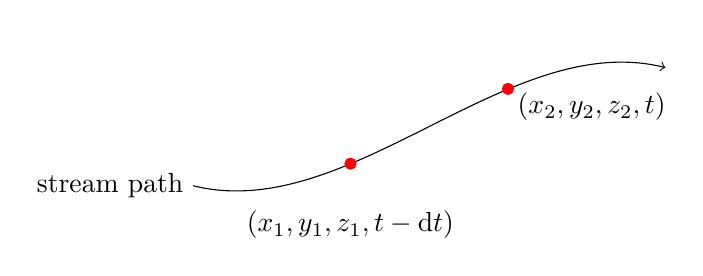
\begin{tikzpicture}
        \draw[->] (0,1) .. controls (2,0.5) and (4,3) .. (6,2.5);
        \node at (0,1) [left] {stream path};
        \node at (2, 0.5) {$(x_1,y_1,z_1,t-\mathrm{d}t)$};
        \filldraw[red] (2,1.28) circle (2pt);
        \filldraw[red] (4,2.23) circle (2pt);
        \node at (4,2) [right] {$(x_2,y_2,z_2,t)$};
    \end{tikzpicture}
\end{figure}

Here's a stream line where a fluid particle moves along. 
The particle's position is $(x_1,y_1,z_1,t-\mathrm{d}t)$ at time $t-\mathrm{d}t$ and $(x_2,y_2,z_2,t)$ at time $t$. 
For $\mathrm{d} t$ is small enough, 
$(x_1,y_1,z_1)$ and $(x_2,y_2,z_2)$ are very close to each other:
\begin{equation}
    (x_2-x_1, y_2-y_1, z_2-z_1) = (u\mathrm{d}t, v\mathrm{d}t, w\mathrm{d}t)
\end{equation}

When ths particle captures a physical quantity $\phi$, 
the variation of $\phi$ at position $(x_2,y_2,z_2)$ is (regardless the variation of $\phi$ in time):
\begin{equation}
    \mathrm{d}\phi = \phi(t) - \phi(t-\mathrm{d}t) = \frac{\partial \phi}{\partial x} u \mathrm{d}t + \frac{\partial \phi}{\partial y} v \mathrm{d}t + \frac{\partial \phi}{\partial z} w \mathrm{d}t
\end{equation}
the equation above declares that the variation of $\phi$ is caused by 
upstream physical quantity $\phi$. 
A time variation of $\phi$ is added as $\frac{\partial \phi}{\partial t}$ in unsteady flow field.

In Lagrangian discription, 
we track the motion of a fluid particle. 
Thus the part $\vec{u}\cdot\nabla\phi$ in the equation above is eliminated. 
Only fixed point in space will feel the change along the direction of flow field.
Thus the equation above is simplified as:
\begin{equation}
    \frac{\mathrm{d} \phi}{\mathrm{d} t} = \frac{\partial \phi}{\partial t}
\end{equation}

We use $\mathrm{D}^L$ and $\mathrm{D}^E$ to represent the variation of $\phi$ in Lagrangian discription and Euler discription respectively:
\begin{equation}
    \begin{aligned}
        \frac{\mathrm{D}^L \phi}{\mathrm{D} t} &= \frac{\partial \phi}{\partial t}\\
        \frac{\mathrm{D}^E \phi}{\mathrm{D} t} &= \frac{\partial \phi}{\partial t} + \vec{u}\cdot\nabla\phi
    \end{aligned}
\end{equation}

\subsection{Fluid Equation in Lagrangian Discription}

\subsubsection{Continuity Equation}

The continuity equation is derived from the conservation of mass. 
Considering a fluid particle with mass $m$ and volume $\delta V$, 
of which the shape is cuboid with $\Delta x$, $\Delta y$ and $\Delta z$ as its edges.
The volume can be represented as:
\begin{equation}
    \delta V = \Delta x \Delta y \Delta z
\end{equation}

\begin{figure}[H]
    \centering
    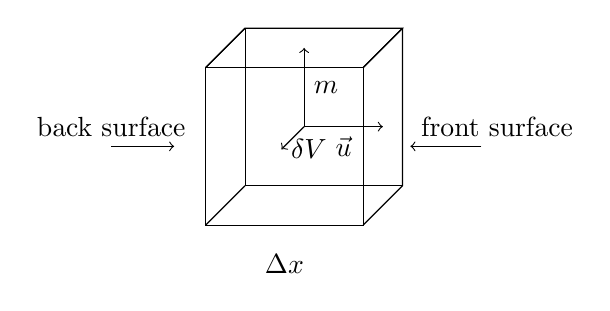
\begin{tikzpicture}
        % draw a cuboid with \delta x, \delta y and \delta z as its edges
        \draw (0,0) -- (0,2) -- (2,2) -- (2,0) -- cycle;
        \draw (0,2) -- (0.5,2.5) -- (2.5,2.5) -- (2,2);
        \draw (2,0) -- (2.5,0.5) -- (2.5,2.5);
        \draw (2.5,2.5) -- (2.5,0.5) -- (0.5,0.5);
        \draw (0.5,0.5) -- (0.5,2.5);
        \draw (0.5,0.5) -- (2.5,0.5);
        \draw (0,2) -- (0.5,2.5);
        \draw (2,2) -- (2.5,2.5);
        \draw (0,0) -- (0.5,0.5);
        % draw the velocity vector
        \draw[->] (1.25,1.25) -- (2.25,1.25);
        \node at (1.75,1.25) [below] {$\vec{u}$};
        % draw the mass vector
        \draw[->] (1.25,1.25) -- (1.25,2.25);
        \node at (1.25,1.75) [right] {$m$};
        % draw the volume vector
        \draw[->] (1.25,1.25) -- (1.25,1.25,0.75);
        \node at (1.25,1.25,0.75) [right] {$\delta V$};
        % front surface
        \node at (3.7,1) [above] {front surface};
        \draw[->] (3.5,1) -- (2.6,1);
        % back surface
        \node at (-1.2,1) [above] {back surface};
        \draw[->] (-1.2,1) -- (-0.4,1);
        % dx
        \node at (1,-0.5) {$\Delta x$};
    \end{tikzpicture}
\end{figure}

The mass of the fluid particle is:
\begin{equation}
    m = \rho \delta V = \rho \Delta x \Delta y \Delta z
\end{equation}

For conservation of mass, 
the variation of mass in the fluid particle is:
\begin{equation}
    \begin{aligned}
        0=\mathrm{d} m &= 
        \mathrm{d} (\rho \Delta x \Delta y \Delta z)\\
        &=
        \Delta x \Delta y \Delta z \mathrm{d} \rho +
        \rho \mathrm{d} (\Delta x \Delta y \Delta z)\\
    \end{aligned}
\end{equation}

In the cuboid model, as the back surface of cuboid moves with speed $u$, 
the front surface of cuboid moves with speed $u+\frac{\partial u}{\partial x}\Delta x$.
Thus the relative speed between the front surface and back surface is $\frac{\partial u}{\partial x}\Delta x$.
With a duration of $\mathrm{d} t$, 
the cuboid's length along $x$ direction will be changed from $\Delta x$ to:
\begin{equation}
    \Delta x\to 
    \Delta x + \frac{\partial u}{\partial x} \Delta x \mathrm{d} t
    = \Delta x (1 + \frac{\partial u}{\partial x} \mathrm{d} t)
\end{equation}
denote $\epsilon_i = \frac{\partial u_i}{\partial x_i}\mathrm{d} t$, 
we will have:
\begin{equation}
    \Delta x_i \to \Delta x_i (1+\epsilon_i)
\end{equation}
and the volume derivation during $\mathrm{d} t$ is:
\begin{equation}
    \begin{aligned}
        \mathrm{d} (\Delta x \Delta y \Delta z) &=
        \Delta x \Delta y \Delta z (1+\epsilon_x)(1+\epsilon_y)(1+\epsilon_z) - \Delta x \Delta y \Delta z\\
        &=
        \Delta x \Delta y \Delta z (\epsilon_x + \epsilon_y + \epsilon_z)\\
        &=
        \Delta x \Delta y \Delta z \nabla\cdot\vec{u} \mathrm{d} t
    \end{aligned}
\end{equation}
substitute the equation above into the equation of mass conservation:
\begin{equation}
    \delta V \mathrm{d}\rho + \rho \delta V \nabla \cdot \vec{u} \mathrm{d} t = 0
\end{equation}

Finally, we have the continuity equation in Lagrangian discription:
\begin{equation}
    \frac{\mathrm{D}^L \rho}{\mathrm{D} t} + \rho \nabla \cdot \vec{u} = 0
\end{equation}
which is usually written as:
\begin{equation}
    \frac{\partial \rho}{\partial t}=-\rho \nabla \cdot \vec{u}
\end{equation}

\subsubsection{Momentum Equation}

The momentum equation is derived from Newton's law.
Considering a fluid particle with mass $m$ and volume $\delta V$,
the external force acting on the fluid particle is $\vec{f}$:
\begin{equation}
    m\frac{\mathrm{D}^L \vec{u}}{\mathrm{D} t} = \vec{f}
\end{equation}

The external force $\vec{f}$ can be decomposed into two parts, 
one is the body force $\vec{f}_b$ and the other is the surface force $\vec{f}_s$:
\begin{equation}
    \vec{f} = \vec{f}_b + \vec{f}_s
\end{equation}

For body force, which is usually gravity, electric force, magnetic force, etc., 
the force is proportional to the mass of the fluid particle:
\begin{equation}
    \vec{f}_b = m \vec{g}
\end{equation}

Surface force is usually more complicated. 
Under Stokes assumption, 
the surface foce acting on $j$-th surface along direction $i$'s $\tau_{ij}$ is:
\begin{equation}
    \tau_{ij} = (-p + \lambda\nabla\cdot\vec{u})\delta_{ij} 
    + \mu\left(\frac{\partial u_i}{\partial x_j} + \frac{\partial u_j}{\partial x_i}\right)
\end{equation}
what's more, Stokes assumption requires that in steady flow field, 
the pressure force is equal to the surface force:
\begin{equation}
    \tau_{11}+\tau_{22}+\tau_{33} = -3p 
    + 3\lambda\nabla\cdot\vec{u} 
    + 2\mu \nabla \cdot \vec{u}
    \to
    \lambda = -\frac{2}{3}\mu
\end{equation}

Thus the surface force is:
\begin{equation}
    \vec{f}_s = \nabla\cdot [\tau]
    = 
    -\nabla p + \mu \nabla^2 \vec{u} + \frac{\mu}{3}\nabla(\nabla\cdot\vec{u})
\end{equation}
equation above requires that $\mu$ is constant in fluid field. 
Moreover, when we discuss a incompressible fluid, 
$\frac{\mu}{3}\nabla(\nabla\cdot\vec{u})$ is eliminated.

Finally, we have the momentum equation in Lagrangian discription:
\begin{equation}
    \frac{\mathrm{D}^L \vec{u}}{\mathrm{D} t} = - \frac{1}{\rho}\nabla p + \frac{\mu}{\rho}\nabla^2\vec{u} + \vec{g}
\end{equation}
which is usually written as:
\begin{equation}
    \frac{\partial \vec{u}}{\partial t} = - \frac{1}{\rho}\nabla p + \frac{\mu}{\rho}\nabla^2\vec{u} + \vec{g}
\end{equation}

\subsubsection{Energy Equation}

SPH method usually focus on motion of incompressible fluid like water, 
energy equation is not necessary in this case. 
I will finish this part later.

\subsubsection{Equation of State}

In SPH method, 
the equation of state is largely depend on the scheme. 
A large widely used scheme is weakly compressible scheme:
\begin{equation}
    \label{eq:Weakly Compressible Scheme}
    p = \frac{c_0^2\rho_0}{\gamma}
    \left[
        \left(\frac{\rho}{\rho_0}\right)^\gamma - 1
    \right]
\end{equation}
when $\rho-\rho_0$ is small enough, 
the equation above can be simplified as:
\begin{equation}
    \begin{aligned}
        p &= \frac{c_0^2\rho_0}{\gamma}
        \left[
            \left(1+\frac{\rho-\rho_0}{\rho_0}\right)^\gamma - 1
        \right]\\
        &\approx \frac{c_0^2\rho_0}{\gamma}
        \left[
            1 + \gamma\frac{\rho-\rho_0}{\rho_0} - 1
        \right]\\
        &= c_0^2 (\rho - \rho_0)
    \end{aligned}
\end{equation}

In SPHysics, and Monaghan's SPH method, $\gamma=7$ and $c_0$ is 
an artificial speed of sound, which is usually set to $10\max\{U_{\max},\sqrt{gL_{\max}}\}$.

\subsection{SPH Discretization}

\subsubsection{Spatial Discretization}

In this section, 
we only consider restrict formula of SPH discretization. 
Tricks like artificial viscosity, XSPH, kernel correction, etc. 
will be discussed in the next section.

As is discussed above, 
fluid equation in Lagrangian discription can be discretized as:
\begin{equation}
    \begin{aligned}
        \left(\frac{\partial\rho}{\partial t}\right)_i
        &=
        \sum_j m_j \vec{u}_{ij} \cdot \nabla W_{ij}\\
        \left(\frac{\partial\vec{u}}{\partial t}\right)_i
        &=
        -\sum_j m_j \left(\frac{p_i}{\rho_i^2} + \frac{p_j}{\rho_j^2}\right) \nabla W_{ij} + 
        \vec{g} + 
        \sum_j \frac{4m_j(\mu_i+\mu_j)\vec{r}_{ij}\cdot \nabla W_{ij}}{(\rho_i+\rho_j)^2[r_{ij}^2+(0.1h)^2]}\vec{u}_{ij}\\
        \left(\frac{\partial \vec{x}}{\partial t}\right)_i
        &=
        \vec{u}_i
    \end{aligned}
\end{equation}

\subsubsection{Time Discretization}

For each step needs a neighbour search over all particles.
Thus traditional Runge-Kutta method is not suitable for SPH method.

Current code uses explicit Euler method. 
Another widely used method is predictor-corrector method,
which will added in future work.

CFL number is used to control the time step.
A conservative time step is:
\begin{equation}
    \Delta t=\frac{h}{10c_0}
\end{equation}

As $U_{\max}$ is usually smaller than $0.1c_0$,
each time step only allows a particle to move a distance of $0.01h$ in this format.

\subsection{Boundary Condition}

\subsubsection{Compulsive Wall Boundary Condition}

Monaghan in his paper 'Solitary Waves on a Cretan Beach' first proposed the conpulsive boundary condition.
He aranged a series of fixed wall particles on the boundary of the fluid field 
which will have a compulsive force on the fluid particles.

\begin{figure}[H]
    \centering
    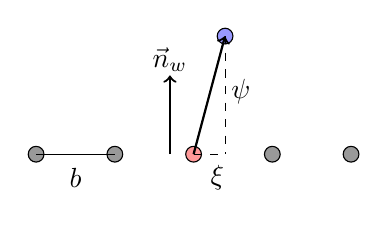
\begin{tikzpicture}
        \foreach \x in {0,1,3,4}
        \draw[fill=black!40!white, draw=black] (\x,0) circle (0.1);
        \draw[fill=blue!40!white, draw=black] (2.4,1.5) circle (0.1);
        \draw[fill=red!40!white, draw=black] (2,0) circle (0.1);
        
        \draw[->, thick] (2,0) -- (2.4,1.5);
        \draw[->, thick] (1.7,0) -- (1.7,1);
        \node at (1.7,1.2) {$\vec{n}_w$};
        \draw[dashed] (2.4,1.5) -- (2.4,0);
        \draw[dashed] (2, 0) -- (2.4,0);

        \draw[-] (0,0)--(1,0);
        \node at (0.5, -0.3) {$b$};

        \node at (2.6,0.8) {$\psi$};
        \node at (2.3, -0.3) {$\xi$};
    \end{tikzpicture}
\end{figure}

With wall particle's gap $b$ and normal vector $\vec{n}_w$, 
considering a fluid particle's position at $(\xi, \psi)$ relative to a wall particle, 
it will feel a compulsive force $\vec{f}_w$:
\begin{equation}
    \vec{f}_w=P(\psi)R(\xi)\epsilon(u_{\perp},z)\vec{n}_w
\end{equation}

$\psi$ is the distance between the fluid particle and the wall particle,
$\xi$ is the projection of the fluid particle on the wall particle.

The part $P(\psi)$ is the compulsive force caused by the distance between the fluid particle and the wall particle.
It is designed to be a function with singularity at $\psi=0$:
\begin{equation}
    P(\psi)=A\frac{1}{\sqrt{q}}(1-q)
\end{equation}
in which $A=\frac{1}{h}(0.1c_i)^2$ and $q=\frac{\psi}{2h}$.
$c_i$ is the artificial speed of sound in fluid particle $i$.
Although the equation is proved wrong in my personal practice, 
I will discuss it later.

The part $R(\xi)$ is the compulsive force caused by the projection of the fluid particle on the wall particle.
It is designed to be a periodic function:
\begin{equation}
    R(\xi)=\frac{1}{2}\left[
        1+\cos\left(\frac{2\pi\xi}{b}\right)
    \right]
\end{equation}

However, as I practice the compulsive boundary condition, still particles will 
penetrate the wall. I fix this problem by analysing the characteristic of cosine function.
\begin{figure}[H]
    \centering
    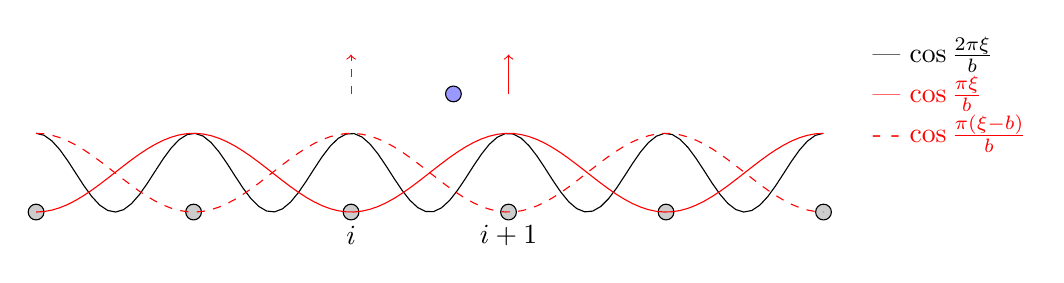
\begin{tikzpicture}
        \foreach \x in {-3,-2,-1,0,1,2}
        \filldraw[fill=gray!40!white, draw=black] (2*\x,0) circle (0.1);
        % plot cos 2pi x
        \draw[domain=-3:2,samples=100] plot (\x*2,{0.5+0.5*cos(360*\x)});
        % plot cos pi x
        \draw[domain=-3:2,samples=100,red] plot (\x*2,{0.5+0.5*cos(180*\x)});
        \draw[domain=-3:2,samples=100,red,dashed] plot (\x*2,{0.5+0.5*cos(180*(\x-1)});
        % fluid particle
        \filldraw[fill=blue!40!white, draw=black] (-0.7,1.5) circle (0.1);
        
        \draw[->,red] (0,1.5)--(0,2.0);
        \draw[->,red,dashed] (-2,1.5)--(-2,2.0);

        \node[right] at (4.5,2) {---  $\cos \frac{2\pi\xi}{b}$};
        \node[right,red] at (4.5,1.5) {---  $\cos \frac{\pi\xi}{b}$};
        \node[right,red] at (4.5,1) {- -  $\cos \frac{\pi(\xi-b)}{b}$};

        \node at (-2, -0.3) {$i$};
        \node at (0, -0.3) {$i+1$};
    \end{tikzpicture}
\end{figure}

As is shown in the figure above,
a fluid particle is influenced by 2 wall particles,
one is the wall particle at $\xi$ and the other is the wall particle at $b-\xi$.
\begin{equation}
    \begin{aligned}
        R_{i} &= \frac{1}{2}\left[
            1+\cos\left(\frac{\pi\xi}{b}\right)
        \right]\\
        R_{i+1} &= \frac{1}{2}\left[
            1+\cos\left(\frac{\pi(b-\xi)}{b}\right)
        \right]\\
        R_{i}+R_{i+1} &= 1+\frac{1}{2}\left[
            \cos\left(\frac{\pi\xi}{b}\right) + \cos\left(\frac{\pi(b-\xi)}{b}\right)
        \right]=1
    \end{aligned}
\end{equation}
this will garantee that a particle fly along the wall feels a constant compulsive force.
However, 
if use equation in SPHysics documnent and Delong Xu's book or Rogers's paper, 
the compulsive force will be:
\begin{equation}
    \begin{aligned}
        R_{i} &= \frac{1}{2}\left[
            1+\cos\left(\frac{2\pi\xi}{b}\right)
        \right]\\
        R_{i+1} &= \frac{1}{2}\left[
            1+\cos\left(\frac{2\pi(b-\xi)}{b}\right)
        \right]\\
        R_{i}+R_{i+1} &= 1+\frac{1}{2}\left[
            \cos\left(\frac{2\pi\xi}{b}\right) + \cos\left(\frac{2\pi(b-\xi)}{b}\right)
        \right]=1+\cos\left(\frac{2\pi\xi}{b}\right)
    \end{aligned}
\end{equation}

When $\xi=\frac{b}{2}$, $R_{i}+R_{i+1}=0$. 
When $\xi=0$, $R_{i}+R_{i+1}=2$, which is twice of the compulsive force at $\xi=\frac{b}{2}$.
This indicates that a fluid particle will penetrate the wall in the middle of two wall particles 
but will be pushed back when it is close to a wall particle.
After all, I modify this equation to:
\begin{equation}
    R(\xi)=\frac{1}{2}\left[
        1+\cos\left(\frac{\pi\xi}{b}\right)
    \right]
\end{equation}

A coefficient $\epsilon(u_{\perp},z)$ is added to the compulsive force to 
modify the compulsive force when the fluid particle is close to the wall.

\begin{equation}
    \epsilon(u_{\perp},z)=\epsilon (u_{\perp})+\epsilon(z)
\end{equation}
其中:
\begin{equation}
    \epsilon(u_{\perp})=
    \begin{cases}
        0 &\quad u_{\perp}\geq 0\\
        -\frac{20u_{\perp}}{c_0} &\quad -20u_{\perp}<c_0\\
        1 &\quad -20u_{\perp}\geq c_0
    \end{cases}
\end{equation}
\begin{equation}
    \epsilon(z)=
    \begin{cases}
        0 &\quad z\geq 0\\
        -\frac{z}{h_0} &\quad -h_0<z<0\\
        1 &\quad -h_0\geq z
    \end{cases}
\end{equation}
where $h_0$ is the depth of the location of the wall particle. 
$\epsilon(z)$ is a modification to pressure depth.
And $u_{\perp}$ is the velocity of the fluid particle along the normal vector of the wall particle.
$\epsilon(u_{\perp})$ is a modification to the velocity of the fluid particle along the normal vector of the wall particle.

In Monaghan's paper, 
$(0.1c_i)^2$ can be used as $\frac{|p|}{\rho}$, 
which is the pressure depth of the fluid particle. 
And the coefficient $\epsilon$ can be used in another form by Monaghan:
\begin{equation}
    A=\frac{1}{h}(0.01c^2 -\beta c\vec{u}_i\cdot\vec{n}_w)
\end{equation}
where:
\begin{equation}
    \beta=
    \begin{cases}
        \begin{aligned}
            0 &\quad \vec{u}_i\cdot\vec{n}_w\geq 0\\
            1 &\quad \vec{u}_i\cdot\vec{n}_w<0
        \end{aligned}
    \end{cases}
\end{equation}

\subsubsection{Open Boundary Condition}

Open boundary condition is widely applied in traditional CFD method.
However, 
SPH method will face difficulty when open boundary condition is applied for
there will be particles flying out of and flying into the fluid field.
This means that the fluid field's particle number is varying within time, 
which cause trouble in coding.

I will finish this in future work.

\subsubsection{Other Boundary Conditions}

Other boundary conditions.